% R2MT-Net manuscript draft prepared with the official MDPI LaTeX class.
% Main file for Overleaf: manuscript.tex

\documentclass[electronics,article,submit,oneauthor]{Definitions/mdpi}

%=================================================================
% MDPI metadata
\firstpage{1}
\makeatletter
\setcounter{page}{\@firstpage}
\makeatother
\pubvolume{1}
\issuenum{1}
\articlenumber{0}
\pubyear{2026}
\copyrightyear{2026}
\datereceived{}
\daterevised{}
\dateaccepted{}
\datepublished{}

%=================================================================
% Local commands
\newcommand{\modelname}{R\textsuperscript{2}MT-Net}
\graphicspath{{figures/}}

%=================================================================
% Front matter. Add the author's complete postal address and ORCID before submission.
\Title{\modelname: An OCR-Enabled End-to-End Pointer-Gauge Reader with Multi-Risk Moment Transport}

\Author{Xiaoyi Liang $^{1,}$*}
\AuthorNames{Xiaoyi Liang}

\address{%
$^{1}$ \quad University College London, London, UK; ucabx23@ucl.ac.uk}

\corres{Correspondence: ucabx23@ucl.ac.uk}

% Approximately 200 words; objective claims only.
\abstract{Off-axis pointer-gauge images alter dial support and pointer-to-scale relations. We propose \modelname, an OCR-enabled image-to-physical-reading system with a shared ResNet-18, relation-encoded dual-observation transport, three risk-specialized moment heads, conservative representation-conditioned arbitration, and one final moment-exact posterior tilt. On a retrospective 1,558-image, 14-scene SyncG evaluation, three fitted models achieved $1.0517\pm0.0415$\%FS normalized mean absolute error (NMAE) across six conditions and $1.3099\pm0.0501$\%FS in the projective pool, 24.53\% and 33.58\% below a matched EfficientNet-B0 endpoint. On 1,395 industrial regions of interest, \modelname\ reduced projective NMAE from $28.1866\pm2.7176$\%FS for Direct-ResNet18 to $21.5524\pm3.7915$\%FS (paired reduction 6.6342 percentage points; 95\% confidence interval, 4.3215--8.8624). EfficientNet-B0 reached $18.0914\pm2.9211$\%FS on the same industrial projective pool, revealing a backbone-dependent domain reversal rather than universal superiority. On a 774-row same-pixel intersection, \modelname\ obtained $0.9054\pm0.0392$\%FS versus 1.6444\%FS for an annotation-assisted vector detection network reference. Accepted-sample OCR accuracy within 5\%FS was $74.07\pm12.83$\% ($n=9$). Model-only RTX 4060 latency was 22.32 ms at batch 1. These retrospective results support projective-specific transport; independent confirmation remains required.}

\keyword{analog gauge reading; pointer meter; projective distortion; risk-specialized learning; moment transport; optical character recognition; industrial vision}

%%%%%%%%%%%%%%%%%%%%%%%%%%%%%%%%%%%%%%%%%%
\begin{document}

\section{Introduction}
\label{sec:introduction}

Analog pointer gauges remain common in power systems, process plants, laboratories, and legacy industrial equipment. Camera-based reading can automate inspection without modifying the instrument. Previous work has demonstrated mobile-phone transcription, autonomous reading in unstructured environments, and robot-deployable gauge-reading pipelines \cite{howells2021analogue,milana2022gauges,reitsma2024underpressure}. The engineering objective is therefore not merely pointer localization, but an end-to-end mapping from a field photograph to a physical reading.

Projective distortion is a central obstacle. An oblique view changes apparent dial support, compresses angular intervals non-uniformly, alters sampling density inside the detector crop, and distorts pointer-to-scale relations. Existing systems address parts of this problem through segmentation and perspective correction \cite{tan2024transunet}, prior-guided keypoints \cite{chu2025prikmet}, or virtual-point pose rectification \cite{lee2026p2yolo}. Vector representations reduce dependence on complete pointer masks \cite{dong2021vdn}, while reconstruction models target occlusion \cite{ninama2026grnet}. These approaches show that geometry matters, but an operational reader must still decide how evidence from an original and a normalized observation should change an individual reading.

Our completed ablation indicates a residual gap after any one risk-specialized correction because the observed errors are heterogeneous. Mean-error optimization emphasizes the majority of samples; a tail objective protects large errors; and condition weighting prioritizes the severe perspective-plus-blur case. In this study these objectives are complementary rather than interchangeable. A fixed multi-risk prior captures most of the measured complementarity, while sample-level routing provides only a smaller conservative refinement. Probability-space fusion must also be controlled: mixing several transported posteriors can combine their shapes before one coherent target moment has been established.

We therefore propose \modelname, an optical character recognition (OCR)-enabled end-to-end reader. Its progress core first constructs original and support-normalized observations. One shared ResNet-18 \cite{he2016resnet} supplies endpoint posteriors, final 512-dimensional representations, and stride-8/16 features. A relation-transport block aligns the feature hierarchies, explicitly encodes signed discrepancy, absolute discrepancy, agreement, support, and homography evidence, and produces one base posterior. Three relative-context moment-transport (RCMT) heads then estimate bounded residuals specialized for mean, tail, and combined-condition risk. A compact representation-conditioned router conservatively adjusts a global risk prior. The selected residual is applied to the full base posterior through one moment-exact information projection.

The progress core is integrated into a complete image-to-reading graph. Meter localization supplies a region of interest (ROI); \modelname\ estimates normalized progress; an OCR branch recognizes the ordered range endpoints; and both outputs are converted to physical units. Normalized progress and numeric range recognition solve different visual problems, but both are necessary for a field reading. The present revision reports fresh, checkpoint-matched industrial, OCR-accepted, component-comparison, repeatability, and efficiency replays. OCR performance is limited to accepted-sample accuracy. To keep claims separable, the evidence is organized as an external backbone comparison, relation/risk module ablation, four-model industrial transfer, same-pixel external-method comparison, and matched engineering efficiency.

The completed evidence uses 14,442 SyncG images from 131 scene groups for fitting and 1,558 images from 14 different scene stems for retrospective evaluation \cite{deng2026syncg}. Across three fitted seeds, \modelname\ achieved $1.0517\pm0.0415$\%FS NMAE across six conditions and $1.3099\pm0.0501$\%FS under the three projective conditions. A separate 1,395-ROI industrial replay showed strong paired improvement over Direct-ResNet18 under projection, but also exposed better aggregate transfer by EfficientNet-B0. Both cohorts have historical development use; the reported evidence is therefore retrospective rather than a formal untouched confirmation.

The contributions are as follows:
\begin{enumerate}[leftmargin=*]
    \item To close the gap between normalized pointer progress and a usable physical reading, we develop an OCR-enabled end-to-end architecture with \modelname\ as its single progress core and an explicit conversion using recognized range endpoints.
    \item To address support and pointer-to-scale inconsistency under projection, we introduce a shared dual-observation encoder and relation-encoded moment transport that uses aligned multi-scale features, common support, and homography evidence, with an exact raw-view fallback when the relation is unavailable.
    \item To address heterogeneous mean, tail, and severe-condition errors that one correction objective cannot cover simultaneously, we introduce three risk-specialized moment heads and conservative representation-conditioned arbitration around a fixed prior.
    \item To prevent probability-shape averaging from obscuring one coherent correction, we combine bounded first-moment residuals before one exact posterior transport. Matched module-switch ablations, identity fallback behavior, and paired scene-bootstrap intervals evaluate the four design claims.
\end{enumerate}

\section{Materials and Methods}
\label{sec:methods}

\subsection{Task Definition and End-to-End Scope}
\label{subsec:task}

Let $y$ denote a physical reading and $s_{\min}$ and $s_{\max}$ the ordered endpoints of its meter range. The trainable reader predicts normalized progress
\begin{equation}
p=\frac{y-s_{\min}}{s_{\max}-s_{\min}}\in[0,1].
\label{eq:normalized_progress}
\end{equation}
At system level, localization supplies an ROI, \modelname\ estimates $\hat p$, and the OCR branch supplies $\hat s_{\min}$ and $\hat s_{\max}$. After endpoint-order and unit-consistency checks, the physical output is
\begin{equation}
\hat y=\hat s_{\min}+\hat p(\hat s_{\max}-\hat s_{\min}).
\label{eq:physical_reading}
\end{equation}

The OCR branch retains the existing PP-OCRv4 recognizer from the lightweight PP-OCR family \cite{du2020ppocr}; local inference uses RapidOCR and ONNX Runtime \cite{rapidocr2026}. Detected text regions and start/end-point geometry are combined to decode ordered range endpoints. Figure~\ref{fig:ocr_pipeline} specifies this retained inference structure. The completed replay uses cached detector boxes, the frozen OCR/range decoder, and fresh progress predictions from all three \modelname\ checkpoints. Consequently, we report physical-reading accuracy only for labeled frames that pass the range-validity checks and make no claim about live detector recall or latency.

\begin{figure}[H]
\centering
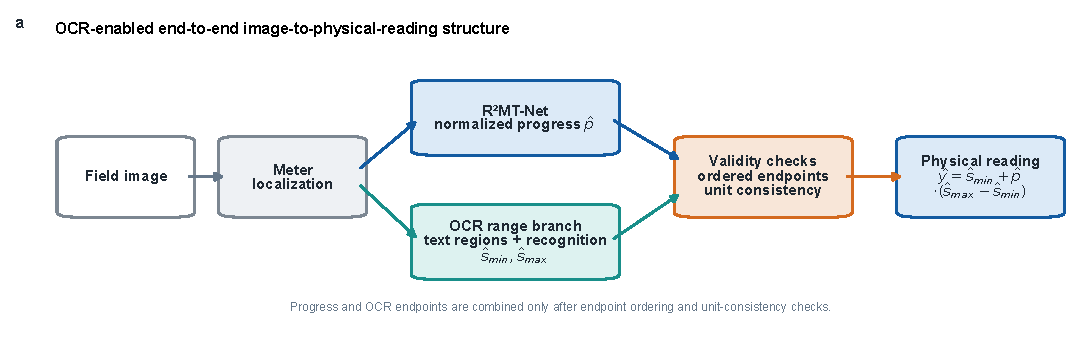
\includegraphics[width=\textwidth]{r2mt_ocr_pipeline.pdf}
\caption{OCR-enabled image-to-physical-reading structure. Localization provides one ROI to the \modelname\ progress path and the OCR range path. Ordered range endpoints and normalized progress are combined only after validity checks. OCR is retained as a system component rather than treated as the paper's primary contribution.}
\label{fig:ocr_pipeline}
\end{figure}

\modelname\ represents progress by a posterior $\mathbf q\in\Delta^{K-1}$ over $x_k=k/(K-1)$, with $K=128$. Its point estimate is the first moment
\begin{equation}
\hat p=\mathbb E_{\mathbf q}[x]=\sum_{k=0}^{K-1}q_kx_k.
\label{eq:posterior_mean}
\end{equation}
The posterior is a constrained computational interface. Its fixed scale is not trained against uncertainty targets; posterior variance is therefore not interpreted as calibrated predictive uncertainty.

\subsection{Data, Scene Separation, and Evidence Status}
\label{subsec:data}

SyncG provides photorealistic synthetic gauges with structural annotations across multiple environments \cite{deng2026syncg}. Scene stems, rather than images, define the separation unit. The fitting roster contains 14,442 images from 131 scene groups. A nested 6,616-image, 60-scene roster supports the initial and refinement passes of the relation transport. The retrospective evaluation contains 1,558 images from 14 different scene stems.

\begin{table}[H]
\caption{Cohorts used in the revised study. Every reported downstream replay uses the three terminal \modelname\ checkpoints without further fitting or adaptation.}
\label{tab:data}
\centering
\small
\begin{tabularx}{\textwidth}{@{}>{\raggedright\arraybackslash}p{0.23\textwidth}>{\raggedright\arraybackslash}p{0.19\textwidth}>{\raggedright\arraybackslash}p{0.19\textwidth}>{\raggedright\arraybackslash}X@{}}
\toprule
\textbf{Cohort} & \textbf{Size} & \textbf{Group unit} & \textbf{Role/status} \\
\midrule
SyncG fitting roster & 14,442 images; 131 scenes & Scene stem & Anchor, refinement, risk-head, and router fitting \\
Nested correction roster & 6,616 images; 60 scenes & Scene stem & Relation-transport initialization and correction refinement \\
SyncG retrospective evaluation & 1,558 images; 14 scenes & Scene stem & Six-condition comparison and ablation \\
Industrial four-model real-photo baseline & 1,395 labeled ROIs; 52 source groups & ROI source group & Six-condition transfer replay for \modelname\ and three raw-image backbones \\
VDN same-pixel intersection & 129 samples; 6 scenes; 774 condition rows & Scene group & Direction-component comparison on identical pixels \\
OCR accuracy subset & 33 labeled full frames; 9 accepted & Photograph & Conditional physical-reading accuracy after validity checks \\
Natural-repeat cohort & 1,203 retained samples; 1,195 distinct images; 86 reading units; 31 instruments & Instrument and exact reading & Identity-fallback check on clean natural captures \\
\bottomrule
\end{tabularx}
\end{table}

Six deterministic conditions are applied to every evaluation ROI: clean; Gaussian blur with standard deviation 0.0015 or 0.0030 times the image short side; virtual-plane perspective at $25^{\circ}$ or $45^{\circ}$; and $45^{\circ}$ perspective combined with the stronger blur. Yaw versus pitch and rotation sign are fixed by sample identifier and seed. All compared methods receive identical condition pixels. The three projective conditions also define synchronized training triplets for the relation and risk modules.

The 14 evaluation scenes are disjoint from the 131 fitting scenes. However, because this cohort has historical development use, we call it a \emph{retrospective scene-disjoint evaluation}, not a formal untouched holdout.

\subsection{Support-Aware ROI Normalization}
\label{subsec:sarn}

For an original ROI $I_r$, support-aware ROI normalization (SARN) constructs a second observation $I_s$ using only input pixels. Flat and mutually consistent corner regions identify the padding pattern produced by a full-canvas projective transform. Significant non-padding components are merged, their convex hull is inspected, and fixed polygon-approximation scales are searched for a reliable quadrilateral. Acceptance requires boundary-padding coverage of at least 0.90, support area between 0.30 and 0.84 of the canvas, quadrilateral-to-hull area ratio of at least 0.84, overall confidence of at least 0.72, and normalized crop area no greater than 0.92.

When accepted, the support bounding box is cropped with a small margin and resized to the original canvas. SARN returns $I_s$, a valid-support mask $M$, and the exact crop-resize homography $H_{r\rightarrow s}$. If any criterion fails, it returns $I_s=I_r$, $M=\mathbf 1$, $H_{r\rightarrow s}=I_3$, and relation-availability indicator $a=0$. SARN recognizes a specified projected-support pattern; it is not claimed to estimate arbitrary natural camera pose.

\subsection{Shared Anchor and Moment-Exact Posterior Lift}
\label{subsec:anchor}

One ImageNet-1K-initialized ResNet-18 parameter set processes $I_r$ and $I_s$ in separate forward passes \cite{he2016resnet}. The passes share every convolution and batch-normalization parameter while preserving distinct observations. The encoder exposes stride-8 features $F^8\in\mathbb R^{128\times H/8\times W/8}$, stride-16 features $F^{16}\in\mathbb R^{256\times H/16\times W/16}$, and a final 512-dimensional representation $z$. A sigmoid scalar head produces endpoint means $\mu_r$ and $\mu_s$.

Each scalar mean is lifted to a 128-bin posterior without changing the mean. For fixed scale $\sigma=0.025$, define
\begin{align}
b_k(\mu,\sigma)&=\exp\!\left[-\frac{(x_k-\mu)^2}{2\sigma^2}\right], \\
q_k(\lambda)&=\frac{b_k(\mu,\sigma)\exp(\lambda x_k)}{\sum_jb_j(\mu,\sigma)\exp(\lambda x_j)}.
\label{eq:posterior_lift}
\end{align}
Twenty Newton updates solve $\sum_kq_k(\lambda)x_k=\mu$ to numerical tolerance. This yields $q_r$ and $q_s$, whose first moments equal their scalar endpoint predictions. The direct anchor is fitted for 30 fixed epochs with $256\times256$ inputs, batch size 64, Smooth-L1 loss with $\beta=0.05$, AdamW with learning rate $3\times10^{-4}$ and weight decay $10^{-4}$, and cosine annealing.

\subsection{Internal Relation-Transport Foundation}
\label{subsec:base_transport}

This subsection describes the internal computation that produces the base state $(q_b,\mu_b)$ used by \modelname. It is presented as a group of layers inside the proposed network rather than as a second named model.

For each scale $l\in\{8,16\}$, the SARN feature map is mapped back to original feature coordinates with $H_{r\rightarrow s}^{-1}$. The support mask is transformed at the same resolution, and only common valid support is used. A shared $1\times1$ projection maps raw and aligned SARN features to $u_r^l$ and $u_s^l$. The per-location relation tensor is
\begin{equation}
R^l=\left[u_r^l,u_s^l,u_s^l-u_r^l,|u_s^l-u_r^l|,u_r^l\odot u_s^l,M^l,\cos(u_r^l,u_s^l)\right].
\label{eq:relation_tensor}
\end{equation}
The signed difference retains direction, the absolute difference records discrepancy magnitude, the product and cosine terms encode agreement, and $M^l$ excludes padding. Each scale is pooled to a $4\times4$ memory, giving 32 relation tokens.

A 13-feature geometry vector contains eight normalized homography-deviation coefficients, two aligned-support fractions, the endpoint mean difference, the log variance ratio, and the Jensen--Shannon divergence between endpoint posteriors. Layer normalization and a linear projection convert it to one geometry token; the external availability mask suppresses the entire memory when the relation is invalid. The resulting 33-token memory conditions 128 progress-bin queries through a two-layer, four-head decoder with token width 64. Queries contain raw/SARN posterior probabilities, log probabilities, cumulative probabilities, local differences, and normalized progress position.

Two zero-initialized summaries of the decoded tokens are averaged and bounded to produce
\begin{equation}
\delta_b=0.025\tanh(d_b),\qquad
\mu_b=\operatorname{clip}(\mu_s+\delta_b,\epsilon,1-\epsilon).
\label{eq:base_shift}
\end{equation}
The layer then solves
\begin{equation}
q_b=\arg\min_{q\in\Delta^{K-1}}D_{\mathrm{KL}}(q\|q_s)
\quad\mathrm{s.t.}\quad \sum_kq_kx_k=\mu_b.
\label{eq:base_projection}
\end{equation}
The information projection \cite{csiszar1975idivergence} is
\begin{equation}
q_{b,k}=\frac{q_{s,k}\exp(\lambda_bx_k)}{\sum_jq_{s,j}\exp(\lambda_bx_j)},
\label{eq:base_tilt}
\end{equation}
where $\lambda_b$ is found by 20 Newton iterations. If homography validity, common aligned support, or SARN availability fails, the outer branch returns $q_b=q_r$ exactly. This prevents missing geometry from becoming a learned correction signal.

\subsection{Risk-Specialized RCMT Heads}
\label{subsec:experts}

Three RCMT heads have identical architecture but different risk objectives. A shared projection within each head maps $z_r$ and $z_s$ from 512 to 64 dimensions. Let $\phi$ denote this projection and $g\in\mathbb R^{13}$ the geometry vector. Each head receives
\begin{equation}
h=\left[\phi(z_r),\phi(z_s),\phi(z_s)-\phi(z_r),|\phi(z_s)-\phi(z_r)|,
\phi(z_r)\odot\phi(z_s),g,\mu_r,\mu_s,\mu_b,\mu_s-\mu_r,\mu_b-\mu_s\right].
\label{eq:expert_relation}
\end{equation}
A layer-normalized 128-unit GELU multilayer perceptron predicts
\begin{equation}
\delta_i=0.05\tanh(f_i(h)),\qquad i\in\{1,2,3\}.
\label{eq:expert_shift}
\end{equation}
Each head has 78,053 parameters and no image encoder.

For physical sample $j$ under projective condition $c$, let $e_{jc}^{(i)}=|\mu_{b,jc}+\delta_{i,jc}-p_j|$. Each expert minimizes
\begin{equation}
\mathcal L_i=\frac{\sum_{j,c}\omega_{ic}e_{jc}^{(i)}}{\sum_{j,c}\omega_{ic}}
+\tau_i\operatorname{Top}_{25\%}(e^{(i)})
+0.02\mathcal L_{\mathrm{cons}}+10^{-4}\mathbb E[\delta_i^2],
\label{eq:expert_loss}
\end{equation}
where $\mathcal L_{\mathrm{cons}}$ is the mean of three pairwise prediction differences within a complete triplet. The mean-risk head uses $\omega=(1,1,1)$ and $\tau=0.1$; the tail-risk head uses $\omega=(1,1,1)$ and $\tau=0.2$; and the combined-risk head uses $\omega=(1,1,2)$ and $\tau=0.2$. The independently fitted objectives preserve expert disagreement for arbitration.

\subsection{Conservative Representation-Conditioned Arbitration}
\label{subsec:router}

The multi-risk prior is $\pi=(0.475,0.280,0.245)$ for mean, tail, and combined-risk heads. A router consumes the raw/SARN representation relation, geometry, endpoint means, all expert shifts, their pairwise differences, and $|\mu_s-\mu_r|$. A shared 512-to-32 projection forms representation terms, and a 64-unit GELU network outputs logit adjustment $r$. Adaptive and conservative weights are
\begin{align}
\widetilde w&=\operatorname{softmax}(\log\pi+r),\\
w&=\pi+\alpha(\widetilde w-\pi),\qquad \alpha=0.5.
\label{eq:routing_weights}
\end{align}
The interpolation deliberately limits sample-level deviation from the prior.

During router fitting, the anchor, relation transport, and experts are frozen. A soft target is constructed from detached expert errors,
\begin{equation}
t_i=\operatorname{softmax}_i(-e_i/T),\qquad T=0.0025.
\label{eq:route_target}
\end{equation}
The router objective is
\begin{equation}
\mathcal L_{\mathrm{route}}=\mathcal L_{\mathrm{weighted\ L1}}+0.1\mathcal L_{\mathrm{tail}}
+0.02\mathcal L_{\mathrm{cons}}+0.0025\operatorname{CE}(t,\widetilde w)
+0.001D_{\mathrm{KL}}(\widetilde w\|\pi),
\label{eq:router_loss}
\end{equation}
with condition weights $(1,1,1.5)$. The imitation term supplies a sample-specific direction, while the KL term discourages unsupported departures. Because the fixed prior and adaptive routes perform similarly, the router is interpreted as a conservative refinement rather than the dominant source of gain.

\subsection{Single Exact Posterior Transport}
\label{subsec:single_transport}

The experts are not fused by averaging probability distributions. Their bounded moment residuals first define one target,
\begin{equation}
\delta=\sum_{i=1}^{3}w_i\delta_i,\qquad
\mu^*=\operatorname{clip}(\mu_b+\delta,\epsilon,1-\epsilon),
\label{eq:fused_target}
\end{equation}
after which the full base posterior is transported once:
\begin{equation}
q_k^*=\frac{q_{b,k}\exp(\lambda^*x_k)}{\sum_jq_{b,j}\exp(\lambda^*x_j)},
\qquad \sum_kq_k^*x_k=\mu^*.
\label{eq:final_transport}
\end{equation}
This order separates risk arbitration from posterior voting. If relation evidence is unavailable, $\delta=0$ and $q^*=q_b=q_r$ exactly.

Figure~\ref{fig:architecture} summarizes the complete progress reader.

\begin{figure}[H]
\centering
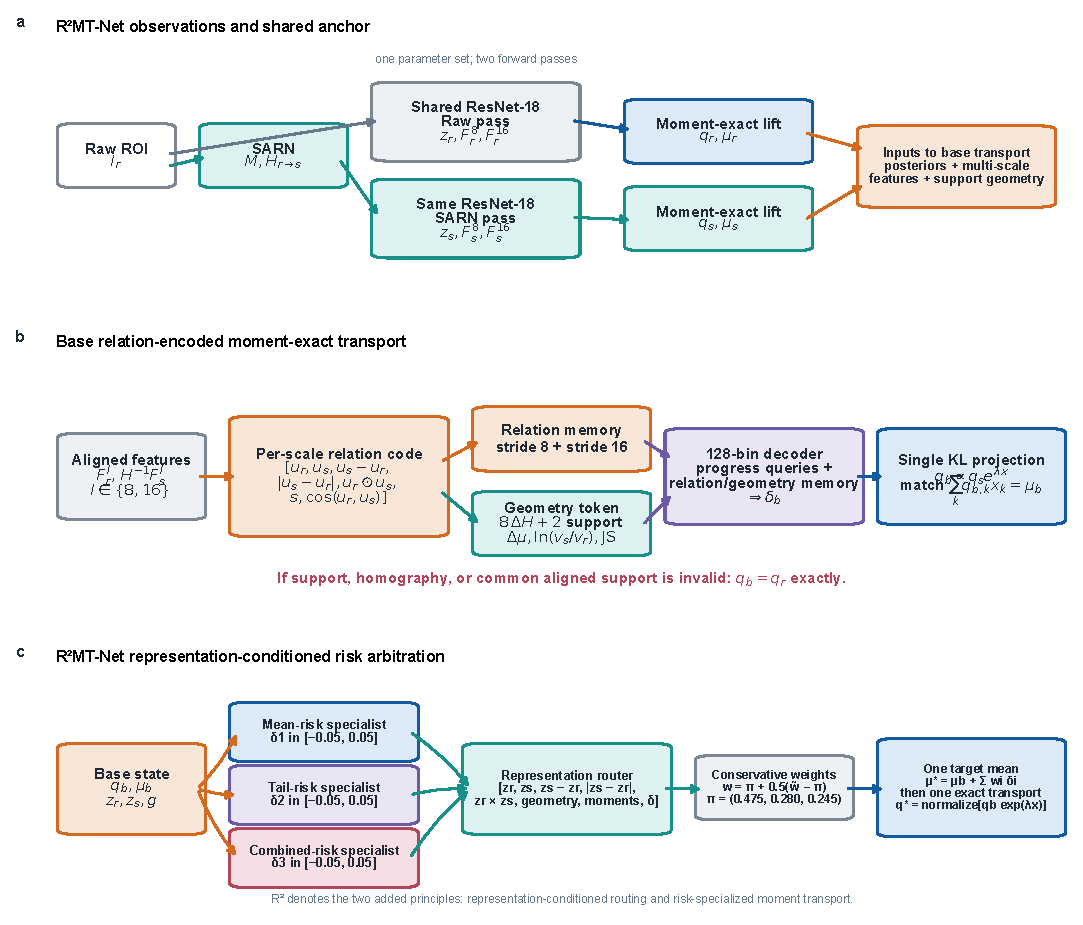
\includegraphics[width=\textwidth]{r2mt_architecture.pdf}
\caption{\modelname\ progress architecture. (\textbf{a}) Original and support-normalized observations are processed by one shared ResNet-18 in two passes and lifted to moment-exact endpoint posteriors. (\textbf{b}) Homography-aligned stride-8/16 features, common support, and target-free geometry condition a 128-bin decoder; an invalid relation returns the raw posterior exactly. (\textbf{c}) Mean-, tail-, and combined-risk RCMT heads estimate bounded moment residuals. Conservative representation-conditioned weights combine the residuals, and one exponential tilt transports the complete base posterior.}
\label{fig:architecture}
\end{figure}

\subsection{Optimization and Parameter Accounting}
\label{subsec:optimization}

The three runs use seeds 20262020, 20262021, and 20262022. All stages use AdamW, cosine annealing, terminal fixed-epoch checkpoints, and no automatic epoch selection on the evaluation cohort. Table~\ref{tab:training_schedule} reports the staged construction. Endpoint and relation refinements retain one shared image encoder and do not add an inference branch.

\begin{table}[H]
\caption{Training schedule and parameter accounting for one fitted \modelname. The refinement sequence is stated for reproducibility rather than presented as a separate model.}
\label{tab:training_schedule}
\centering
\small
\begin{tabularx}{\textwidth}{@{}>{\raggedright\arraybackslash}p{0.24\textwidth}>{\raggedright\arraybackslash}p{0.22\textwidth}>{\raggedright\arraybackslash}p{0.17\textwidth}>{\raggedright\arraybackslash}X@{}}
\toprule
\textbf{Stage} & \textbf{Trainable parameters} & \textbf{Epochs} & \textbf{Fitting population/objective} \\
\midrule
Direct ResNet-18 anchor & 11,177,538 & 30 & 14,442 images; Smooth-L1 scalar progress \\
Endpoint/context refinements & 66,817 added context parameters; no second encoder & $5+2+20$ & Full 14,442 roster; endpoint, layer-4, and 512-D context refinement \\
Relation transport & 180,860 & $5+2+2$ & Nested 6,616 roster; initial fit and two correction refinements \\
Three RCMT heads & $3\times78,053$ & 40 each & Full 14,442 roster as three projective observations; Equation~\eqref{eq:expert_loss} \\
Representation router & 29,777 & 40 & Same cached representations; Equation~\eqref{eq:router_loss}; earlier stages frozen \\
\midrule
Complete \modelname & 11,689,151 unique & -- & One image-encoder parameter set; two observation passes \\
\bottomrule
\end{tabularx}
\end{table}

The initial relation transport uses learning rate $3\times10^{-4}$ and weight decay $10^{-4}$. Each RCMT head uses batch size 256, learning rate $10^{-3}$, and weight decay $10^{-4}$. The router uses the same batch size and optimizer settings. The risk heads and router add 263,936 parameters above the base state and no image encoder.

\subsection{Baselines, Metrics, and Statistics}
\label{subsec:evaluation}

The main comparison uses matched Direct-ResNet18, EfficientNet-B0, and MobileNetV3-Large scalar readers \cite{he2016resnet,tan2019efficientnet,howard2019mobilenetv3}. Each baseline uses the same scene-separated roster, image size, three seeds, terminal fixed-epoch policy, and condition pixels. Their SARN-normalized ledgers were paired by sample identifier and validated pixel identity. The main table contains only external architecture baselines and \modelname; internal construction variants are confined to the ablation.

For targets $p_i$ and predictions $\hat p_i$,
\begin{equation}
\operatorname{NMAE}(\%\mathrm{FS})=100\,N^{-1}\sum_{i=1}^{N}|\hat p_i-p_i|.
\label{eq:nmae}
\end{equation}
Values are reported as arithmetic mean and sample standard deviation across three independently fitted seeds. The projective pool combines the final three conditions.

For preselected ablations, paired effects are comparator absolute error minus \modelname\ absolute error, so positive reduction favors \modelname. Seed-row differences are accumulated within scene stem, and 20,000 nonparametric bootstrap samples resample the 14 scene clusters \cite{davison1997bootstrap}. Intervals quantify paired sampling for completed runs; they do not create an untouched holdout and are not multiplicity adjusted.

\subsection{Downstream Replay Protocols}
\label{subsec:downstream_protocols}

All downstream experiments load the same three terminal \modelname\ checkpoints used in the SyncG table; no fitting, adaptation, checkpoint selection, or automatic retry occurs during these replays. The industrial real-photo baseline contains 1,395 labeled ROIs from 52 provisional source groups. Every ROI receives the same six deterministic conditions as the SyncG evaluation. Direct-ResNet18, EfficientNet-B0, and MobileNetV3-Large are evaluated as raw-image scalar readers on the same source--seed roster and verified identical condition pixels. Means and sample SDs summarize the three independent fits. For paired effects, absolute error is first averaged across seeds within each row; predictions are not ensembled. Twenty thousand bootstrap replicates resample the 52 source groups.

The vector detection network (VDN) comparison uses the set intersection of two independently fixed holdouts: 129 samples from six scene groups, each under six verified pixel-identical conditions, giving 774 rows. Holdout intersection uses identifiers only, not predictions or errors. \modelname\ and SARN plus EfficientNet-B0 are scored from three fitted seeds. The VDN official-200 annotation reference uses one checkpoint and annotation-derived arc information only to convert its direction output to normalized progress. It is therefore a non-deployable direction-component reference rather than an input-equivalent automatic system \cite{dong2021vdn}.

For the OCR replay, the operating point was chosen on a separate 2,224-image public calibration roster without field labels. Cached detector boxes, the frozen OCR/range stack, and fresh three-seed \modelname\ progress predictions are then used on the field frames. The paper reports only conditional accuracy on the nine labeled frames that pass the endpoint-order and range-validity checks; detector recall, end-to-end coverage, and live detector latency are outside this replay's scope.

The natural-repeat check retains 1,203 clean captures representing 1,195 distinct source images, 86 exact-reading units, and 31 physical instruments. It tests the specified identity branch when no projective relation is active. Finally, matched model-only efficiency is measured on an NVIDIA GeForce RTX 4060 with CUDA 12.8, PyTorch 2.11, BF16 autocast, $256\times256$ inputs, batch sizes 1 and 8, 20 warm-up iterations, and 100 timed iterations. Timing includes pinned host-to-device transfer, the required anchor forwards, correction, posterior validation, and final synchronization. It excludes checkpoint construction, image decoding and ROI extraction, SARN materialization, localization, OCR, and accuracy scoring. Shared parameters are counted once.

\section{Results}
\label{sec:results}

\subsection{Backbone-Controlled SyncG Comparison}
\label{subsec:main_results}

Table~\ref{tab:syncg_main} reports the completed six-condition comparison. \modelname\ had the lowest mean NMAE in every displayed condition. Its all-condition NMAE was $1.0517\pm0.0415$\%FS, compared with $1.3935\pm0.0606$ for the strongest external aggregate baseline, EfficientNet-B0, a relative reduction of 24.53\%. In the projective pool, \modelname\ obtained $1.3099\pm0.0501$ versus $1.9722\pm0.0852$\%FS, a 33.58\% reduction.

\begin{table}[H]
\caption{Retrospective SyncG scene-disjoint evaluation. Values are mean $\pm$ sample SD NMAE (\%FS) across three fitted seeds; lower is better.}
\label{tab:syncg_main}
\centering
\scriptsize
\setlength{\tabcolsep}{2.6pt}
\resizebox{\textwidth}{!}{%
\begin{tabular}{lcccccccc}
\toprule
\textbf{Method} & \textbf{Clean} & \textbf{Blur-M} & \textbf{Blur-S} & \textbf{Persp.-25} & \textbf{Persp.-45} & \textbf{45 + blur} & \textbf{All six} & \textbf{Proj. pool} \\
\midrule
Direct-ResNet18 & $0.7910\pm0.0411$ & $0.7932\pm0.0397$ & $0.8207\pm0.0420$ & $1.4422\pm0.0343$ & $2.4302\pm0.0398$ & $2.6219\pm0.0564$ & $1.4832\pm0.0346$ & $2.1648\pm0.0435$ \\
EfficientNet-B0 & $0.8099\pm0.0323$ & $0.8064\pm0.0338$ & $0.8282\pm0.0472$ & $1.4177\pm0.0607$ & $2.1578\pm0.0968$ & $2.3411\pm0.0995$ & $1.3935\pm0.0606$ & $1.9722\pm0.0852$ \\
MobileNetV3-Large & $0.9355\pm0.0435$ & $0.9421\pm0.0489$ & $0.9807\pm0.0385$ & $1.6255\pm0.0489$ & $2.5584\pm0.1962$ & $2.7589\pm0.1664$ & $1.6335\pm0.0716$ & $2.3143\pm0.1361$ \\
\textbf{\modelname} & $\mathbf{0.7829\pm0.0342}$ & $\mathbf{0.7848\pm0.0344}$ & $\mathbf{0.8128\pm0.0409}$ & $\mathbf{1.0295\pm0.0240}$ & $\mathbf{1.3415\pm0.0510}$ & $\mathbf{1.5587\pm0.0757}$ & $\mathbf{1.0517\pm0.0415}$ & $\mathbf{1.3099\pm0.0501}$ \\
\bottomrule
\end{tabular}}
\end{table}

Figure~\ref{fig:core_performance} shows that separation from the three baselines emerges mainly under perspective. Relative to Direct-ResNet18, \modelname\ reduced all-condition and projective NMAE by 29.09\% and 39.49\%; relative to MobileNetV3-Large, the reductions were 35.62\% and 43.40\%.

\begin{figure}[H]
\centering
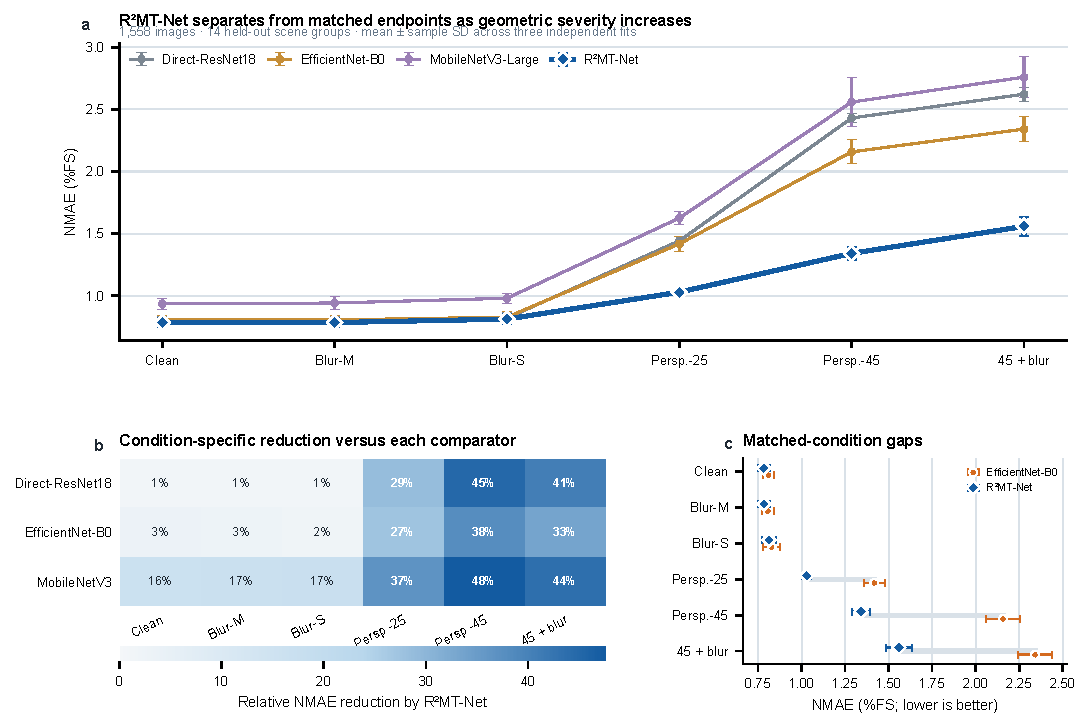
\includegraphics[width=\textwidth]{r2mt_core_performance.pdf}
\caption{Backbone-controlled SyncG comparison. (\textbf{a}) NMAE across all six image conditions; points are three-fit means and error bars are sample SD. (\textbf{b}) Condition-specific relative NMAE reductions achieved by \modelname\ against each comparator. (\textbf{c}) Matched-condition gaps between \modelname\ and EfficientNet-B0.}
\label{fig:core_performance}
\end{figure}

\subsection{Relation Transport, Multi-Risk Necessity, and Fusion Ablation}
\label{subsec:ablation_results}

Table~\ref{tab:ablation} isolates the proposed mechanisms. The internal base relation transport obtained $1.1611\pm0.0424$\%FS across all conditions and $1.5287\pm0.0569$\%FS in the projective pool. The complete multi-risk construction reduced these values by 9.42\% and 14.31\%. In paired scene-bootstrap analysis, the absolute reductions were 0.1094 pp (95\% CI $[0.0898,0.1279]$) and 0.2188 pp ($[0.1805,0.2560]$).

\begin{table}[H]
\caption{Module-switch construction and ablation for \modelname. Values are mean $\pm$ sample SD NMAE (\%FS) across three fitted seeds. For repository traceability only, the first row maps to the internal checkpoint family formerly named ReMST; it is not a second manuscript model.}
\label{tab:ablation}
\centering
\scriptsize
\setlength{\tabcolsep}{3pt}
\resizebox{\textwidth}{!}{%
\begin{tabular}{lcccccc}
\toprule
\textbf{Construction} & \textbf{Relation base} & \textbf{Risk heads} & \textbf{Arbitration} & \textbf{Fusion} & \textbf{All six} & \textbf{Projective pool} \\
\midrule
Base relation transport & On & None & None & Base transport & $1.1611\pm0.0424$ & $1.5287\pm0.0569$ \\
Mean-risk specialist & On & Mean & Single & One transport & $1.0598\pm0.0423$ & $1.3262\pm0.0521$ \\
Tail-risk specialist & On & Tail & Single & One transport & $1.0643\pm0.0373$ & $1.3351\pm0.0412$ \\
Combined-risk specialist & On & Combined & Single & One transport & $1.0669\pm0.0416$ & $1.3403\pm0.0506$ \\
Fixed three-risk prior & On & All three & Fixed & One transport & $1.0520\pm0.0413$ & $1.3105\pm0.0501$ \\
Fully adaptive routing ($\alpha=1$) & On & All three & Adaptive & One transport & $1.0518\pm0.0416$ & $1.3102\pm0.0503$ \\
\textbf{\modelname\ ($\alpha=0.5$)} & \textbf{On} & \textbf{All three} & \textbf{Conservative} & \textbf{One transport} & $\mathbf{1.0517\pm0.0415}$ & $\mathbf{1.3099\pm0.0501}$ \\
\quad without deep representations & On & All three & No deep features & One transport & $1.0533\pm0.0412$ & $1.3132\pm0.0494$ \\
\quad without risk-imitation loss & On & All three & No imitation & One transport & $1.0533\pm0.0416$ & $1.3132\pm0.0502$ \\
\quad posterior probability mixture & On & All three & Conservative & Posterior mixture & $1.1882\pm0.0987$ & $1.5829\pm0.1651$ \\
\bottomrule
\end{tabular}}
\end{table}

No single specialist matched the multi-risk construction. Relative to the best individual head, mean-risk RCMT, \modelname\ reduced all-condition NMAE by 0.0082 pp (95\% CI $[0.0045,0.0119]$) and projective NMAE by 0.0163 pp ($[0.0090,0.0236]$). The fixed prior already captured most of this complementarity: its all-condition NMAE was 1.0520, compared with 1.0517 for the final route. Accordingly, the evidence supports multi-risk arbitration strongly and representation-conditioned adaptation only as an incremental refinement.

Removing deep representations increased all-condition and projective NMAE by 0.0016 pp (95\% CI $[0.0006,0.0028]$) and 0.0033 pp ($[0.0011,0.0057]$). Removing risk imitation produced increases of 0.0016 pp ($[0.0001,0.0032]$) and 0.0033 pp ($[0.0001,0.0065]$).

The largest failure came from changing fusion semantics. Mixing three separately transported posteriors instead of combining their moment residuals before one transport increased all-condition NMAE by 0.1365 pp (95\% CI $[0.0841,0.1963]$) and projective NMAE by 0.2730 pp ($[0.1679,0.3952]$). This is the strongest evidence for separating risk selection from probability aggregation.

\begin{figure}[H]
\centering
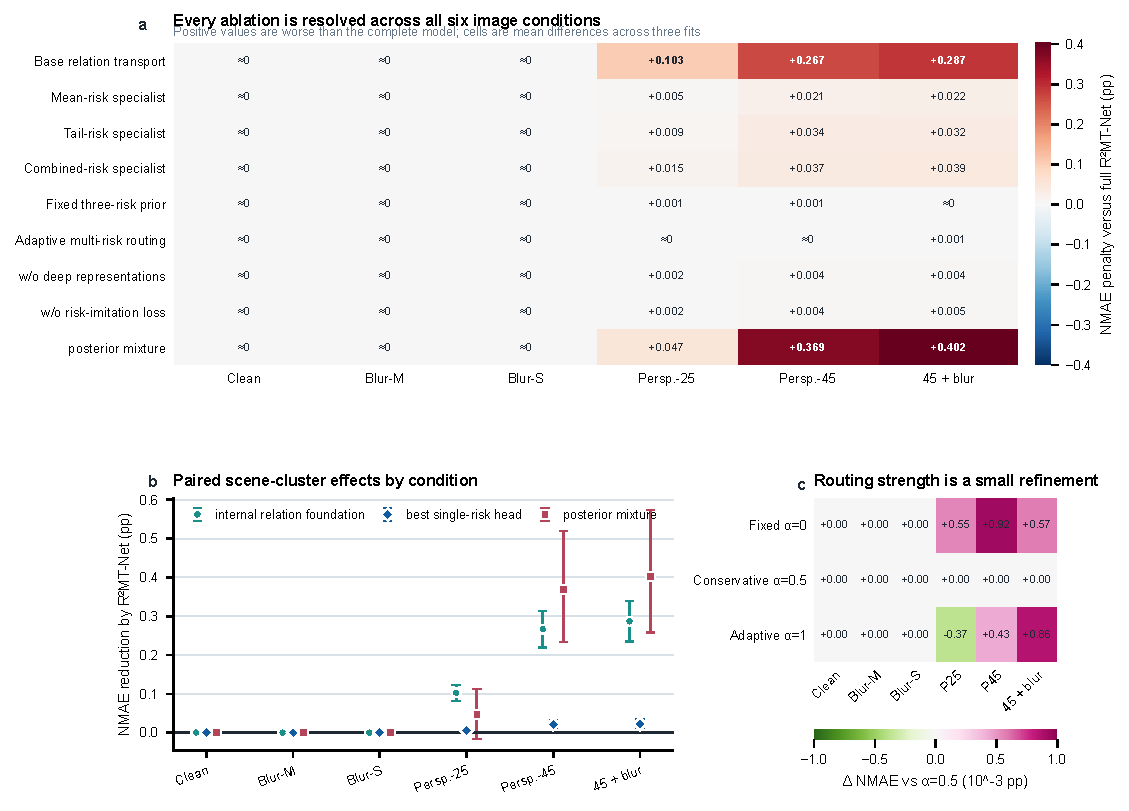
\includegraphics[width=\textwidth]{r2mt_ablation.pdf}
\caption{Relation, risk, and fusion ablations resolved by condition. (\textbf{a}) NMAE penalty of nine construction variants versus complete \modelname\ across all six conditions. (\textbf{b}) Paired scene-cluster effects for the relation foundation, best single-risk specialist, and posterior-mixture variant; positive values favor \modelname. (\textbf{c}) Routing-strength sensitivity relative to conservative $\alpha=0.5$; the $10^{-3}$-percentage-point scale shows that routing is a small refinement.}
\label{fig:ablation}
\end{figure}

\subsection{Industrial Four-Model External Transfer}
\label{subsec:industrial_results}

Table~\ref{tab:industrial} and Figure~\ref{fig:industrial} report all four completed industrial arms. Against the same-backbone Direct-ResNet18 reader, \modelname\ reduced all-condition NMAE from $23.5771\pm2.4504$ to $20.2817\pm3.1514$\%FS, a paired reduction of 3.2954 percentage points (pp; 95\% CI, 2.0864--4.4153). In the projective pool, the reduction was 6.6342 pp (95\% CI, 4.3215--8.8624), from $28.1866\pm2.7176$ to $21.5524\pm3.7915$\%FS. The clean and blur-only effects were near zero, whereas the three projective-condition reductions versus Direct-ResNet18 were 4.0684, 8.4672, and 7.3670 pp, respectively, with all three group-bootstrap intervals excluding zero.

The cross-backbone result is different. EfficientNet-B0 achieved the lowest industrial all-condition and projective-pool means, $15.2550\pm2.3430$ and $18.0914\pm2.9211$\%FS. The all-condition paired effect against EfficientNet-B0 was $-5.0268$ pp (95\% CI, $-8.8278$ to $-1.5108$), while the projective effect was $-3.4611$ pp (95\% CI, $-7.4132$ to 0.2182). Relative to MobileNetV3-Large, \modelname\ was significantly better only at severe $45^{\circ}$ perspective (4.3842 pp; 95\% CI, 0.4246--8.3526); its aggregate intervals crossed zero. Thus, the industrial replay supports the necessity of the proposed projective mechanism relative to a matched Direct-ResNet18 endpoint, but not universal superiority over every backbone. Absolute industrial errors also remain too high to imply deployment-ready accuracy.

\begin{table}[H]
\caption{Four-model industrial real-photo replay. Values are mean $\pm$ sample SD NMAE (\%FS) across three fitted seeds on identical condition pixels; lower is better. Bold marks the lowest column mean.}
\label{tab:industrial}
\centering
\scriptsize
\setlength{\tabcolsep}{3.5pt}
\resizebox{\textwidth}{!}{%
\begin{tabular}{lcccc}
\toprule
\textbf{Method} & \textbf{All six} & \textbf{Projective pool} & \textbf{Persp.-45} & \textbf{45 + blur} \\
\midrule
Direct-ResNet18 & $23.5771\pm2.4504$ & $28.1866\pm2.7176$ & $29.7125\pm2.3260$ & $31.1401\pm3.1682$ \\
\textbf{EfficientNet-B0} & $\mathbf{15.2550\pm2.3430}$ & $\mathbf{18.0914\pm2.9211}$ & $\mathbf{20.3975\pm3.8195}$ & $\mathbf{20.8227\pm3.8398}$ \\
MobileNetV3-Large & $18.7569\pm2.8915$ & $23.2777\pm3.0215$ & $25.6296\pm2.7454$ & $26.3488\pm3.1612$ \\
\modelname & $20.2817\pm3.1514$ & $21.5524\pm3.7915$ & $21.2454\pm3.5084$ & $23.7732\pm4.4467$ \\
\bottomrule
\end{tabular}}
\end{table}

\begin{figure}[H]
\centering
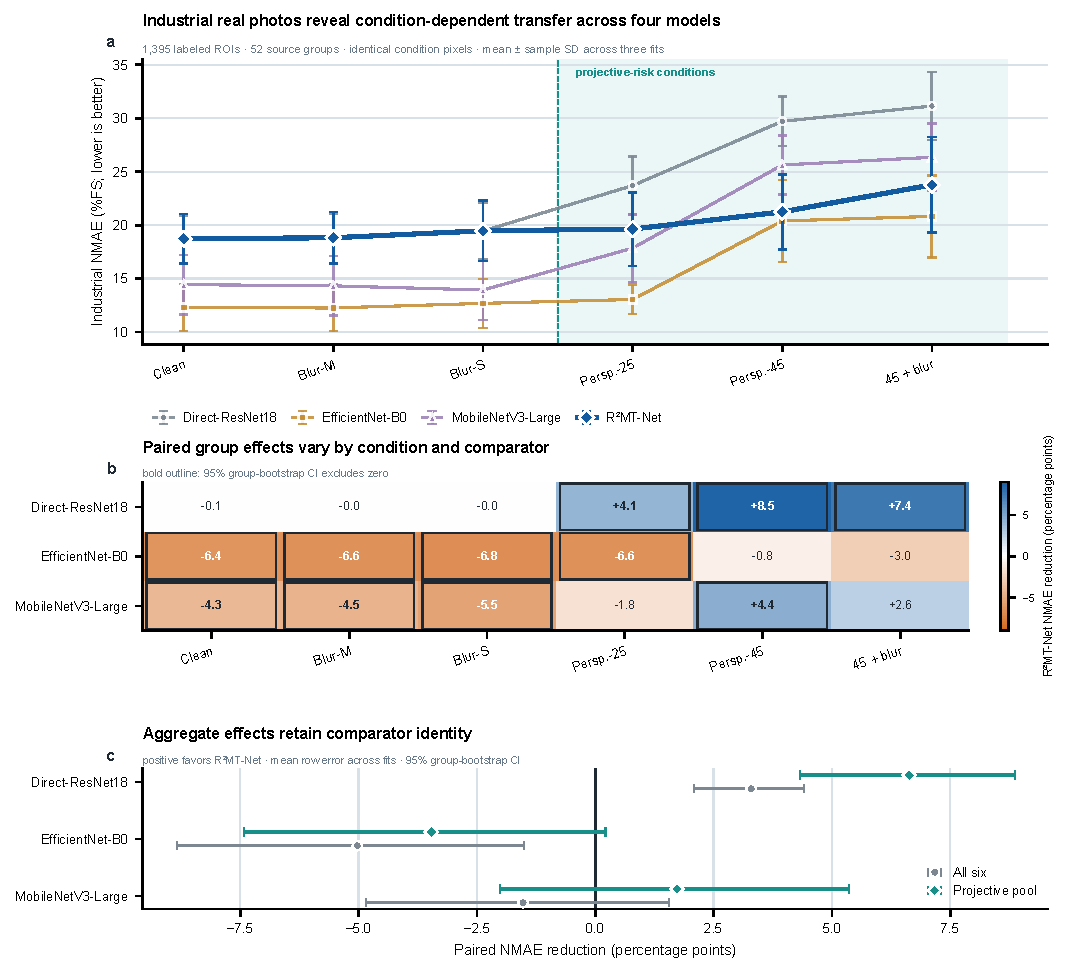
\includegraphics[width=\textwidth]{r2mt_industrial_validation.pdf}
\caption{Industrial transfer across four models. (\textbf{a}) Six-condition NMAE profiles for 1,395 ROIs from 52 source groups; points are three-fit means and error bars are sample SD. (\textbf{b}) Group-paired effects against Direct-ResNet18, EfficientNet-B0, and MobileNetV3-Large. Positive values favor \modelname; outlined cells have 95\% group-bootstrap CIs excluding zero. (\textbf{c}) All-condition and projective-pool paired effects with 20,000-resample 95\% CIs.}
\label{fig:industrial}
\end{figure}

\subsection{Same-Pixel External-Method Comparison}
\label{subsec:vdn_results}

On the 774-row fixed VDN intersection, \modelname\ achieved $0.9054\pm0.0392$\%FS across all conditions, compared with $1.1673\pm0.0638$\%FS for SARN plus EfficientNet-B0 and 1.6444\%FS for the annotation-assisted VDN reference. In the projective pool, the three values were $1.2140\pm0.0714$, $1.7119\pm0.1396$, and 2.1030\%FS. The paired intervals in Table~\ref{tab:vdn} exclude zero for both comparisons. Because the VDN value uses annotation-derived arc information and one checkpoint, this is evidence about the direction component on a fixed same-pixel roster, not an automatic-system ranking.

\begin{table}[H]
\caption{Same-pixel VDN component comparison. NMAE values are in \%FS; three-seed methods are mean $\pm$ sample SD. Paired reduction is comparator minus \modelname\ NMAE in percentage points, with a 20,000-resample scene-group 95\% CI. The VDN annotation reference is a single, non-deployable checkpoint.}
\label{tab:vdn}
\centering
\scriptsize
\setlength{\tabcolsep}{3.2pt}
\resizebox{\textwidth}{!}{%
\begin{tabular}{llccc}
\toprule
\textbf{Metric} & \textbf{Comparison arm} & \textbf{\modelname} & \textbf{Comparator NMAE} & \textbf{Paired reduction (95\% CI)} \\
\midrule
All six & SARN + EfficientNet-B0 & $0.9054\pm0.0392$ & $1.1673\pm0.0638$ & $0.2619\ (0.1231,\ 0.3614)$ \\
Projective pool & SARN + EfficientNet-B0 & $1.2140\pm0.0714$ & $1.7119\pm0.1396$ & $0.4979\ (0.1940,\ 0.6908)$ \\
All six & VDN annotation reference & $0.9054\pm0.0392$ & $1.6444$ & $0.7390\ (0.4207,\ 1.1550)$ \\
Projective pool & VDN annotation reference & $1.2140\pm0.0714$ & $2.1030$ & $0.8890\ (0.3205,\ 1.3742)$ \\
\bottomrule
\end{tabular}}
\end{table}

\begin{figure}[H]
\centering
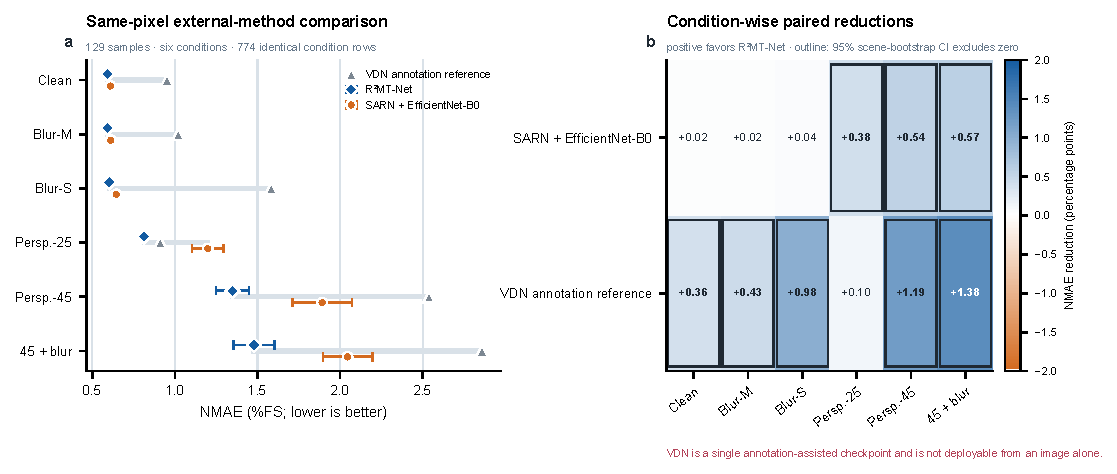
\includegraphics[width=\textwidth]{r2mt_vdn_validation.pdf}
\caption{Same-pixel external-method evidence. (\textbf{a}) Condition-wise NMAE for \modelname, SARN plus EfficientNet-B0, and the annotation-assisted VDN reference on 129 samples and 774 identical condition rows. (\textbf{b}) Condition-wise paired reductions; positive values favor \modelname, and outlined cells have 95\% scene-bootstrap CIs excluding zero.}
\label{fig:vdn}
\end{figure}

\subsection{Identity Fallback and Accepted-Sample OCR Accuracy}
\label{subsec:system_results}

The detector--\modelname--OCR--physical-conversion path achieved an accepted-sample accuracy within 5\%FS of $74.07\pm12.83$\% on the labeled frames that passed the range-validity checks ($n=9$). This value describes accepted outputs only. OCR is retained to complete the image-to-physical-reading graph, but it is not used as evidence for the progress model's main contribution.

Risk-head and routing variants have identical clean and blur-only values because SARN does not declare an active projective relation for those rows. The residual is zero and the model returns its raw-view posterior. Consistently, across 1,203 retained clean natural captures and 86 exact-reading units, \modelname, the raw endpoint, and the SARN endpoint produced identical outputs; the paired NMAE difference was 0 pp with a physical-instrument bootstrap interval of $[0,0]$. This validates identity fallback, not an accuracy gain on non-projective inputs.

\subsection{Model Efficiency}
\label{subsec:efficiency_results}

Table~\ref{tab:efficiency} separates the cost of one raw pass, the second shared-encoder pass, and the complete transport. The full model contains 11.6892 million unique parameters and requires 9.582 registered GFLOPs per sample. Its mean latency was 22.3197 ms at batch 1 and 3.5657 ms per sample at batch 8, corresponding to 44.8 and 280.4 images/s; peak allocated memory was 66.24 and 114.76 MiB. These are model-only measurements, not end-to-end system latency.

\begin{table}[H]
\caption{Matched BF16 model-only efficiency on an RTX 4060. Latency entries are mean/p95 ms per sample over 100 timed iterations after 20 warm-ups. Throughput entries are images/s for batch 1/batch 8. FLOPs cover operators registered by the PyTorch dispatcher.}
\label{tab:efficiency}
\centering
\scriptsize
\setlength{\tabcolsep}{3.5pt}
\resizebox{\textwidth}{!}{%
\begin{tabular}{lccccc}
\toprule
\textbf{Inference arm} & \textbf{Unique parameters (M)} & \textbf{GFLOPs/sample} & \textbf{Batch 1 mean/p95 (ms)} & \textbf{Batch 8 mean/p95 (ms)} & \textbf{Throughput B1/B8} \\
\midrule
Raw-view endpoint & 11.2444 & 4.738 & $4.5619/5.3468$ & $0.9310/1.0162$ & $219.2/1074.1$ \\
Dual-view endpoint & 11.2444 & 9.475 & $8.2589/9.1649$ & $1.8135/1.9096$ & $121.1/551.4$ \\
\textbf{Complete \modelname} & \textbf{11.6892} & \textbf{9.582} & $\mathbf{22.3197/24.4028}$ & $\mathbf{3.5657/3.6734}$ & $\mathbf{44.8/280.4}$ \\
\bottomrule
\end{tabular}}
\end{table}

\begin{figure}[H]
\centering
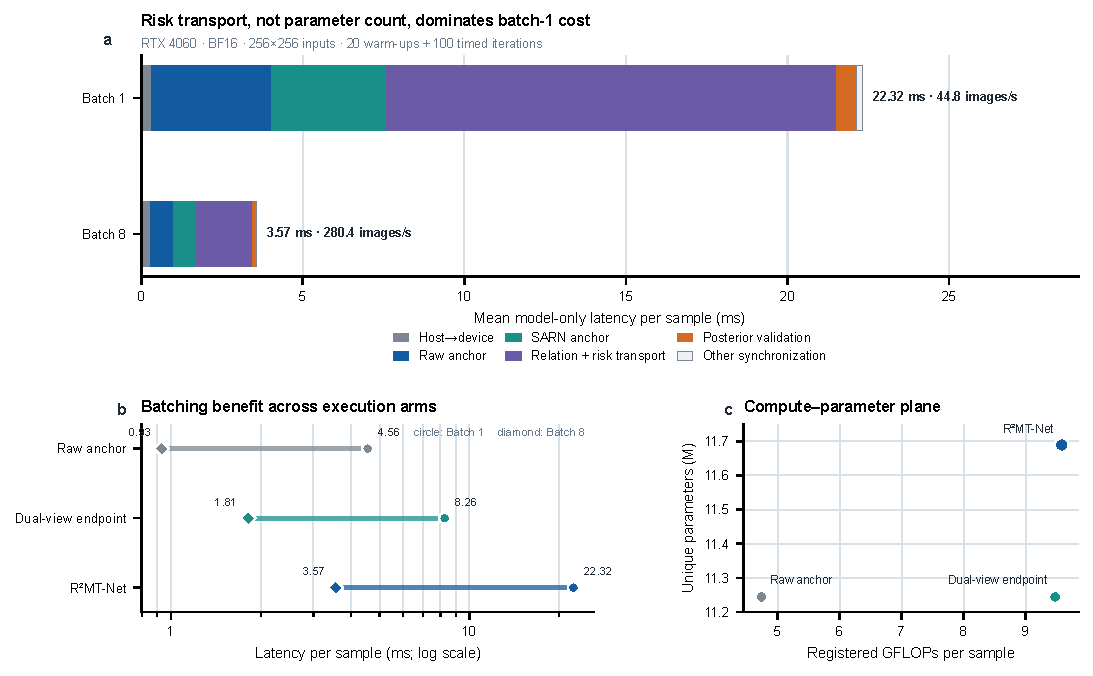
\includegraphics[width=\textwidth]{r2mt_efficiency.pdf}
\caption{Matched model-only efficiency. (\textbf{a}) Stage-stacked mean latency per sample for complete \modelname\ at batch sizes 1 and 8. (\textbf{b}) Batching benefit for the raw anchor, dual-view endpoint, and complete model. (\textbf{c}) Registered GFLOPs versus unique parameter count. Measurements use RTX 4060 BF16 inference; localization, SARN materialization, and OCR are excluded.}
\label{fig:efficiency}
\end{figure}

\section{Discussion}
\label{sec:discussion}

The main empirical need for \modelname\ is heterogeneous risk rather than projective difficulty alone. The complete construction outperformed the base relation transport and each individual specialist. Most of the remaining gain after specialist fitting came from combining complementary risk objectives around a fixed prior; representation-conditioned routing supplied a smaller refinement. This distinction prevents an exaggerated interpretation of the router ablation.

The strongest mechanism result concerns operation order. Posterior probability mixing performed substantially worse than selecting one bounded target moment and transporting the complete base posterior once. A mixture can inherit separated shapes or increased dispersion even when component means are plausible. Equation~\eqref{eq:final_transport} instead gives the minimum-KL update from one reference posterior subject to one mean constraint. This restriction does not guarantee the target is correct, but it defines exactly how expert evidence may change the output.

The internal multi-scale relation path provides reproducible geometric grounding. Original/SARN agreement, discrepancy, support, and homography evidence are explicit; relation availability is testable; and the moment projection connects a decoded residual to a valid posterior. These layers are part of \modelname\ and are not promoted as a separate model in the manuscript.

Compared with explicit geometric rectification \cite{tan2024transunet,lee2026p2yolo}, \modelname\ uses a support-normalized observation and learned cross-view relations rather than claiming general camera-pose recovery. Compared with prior-guided keypoint systems \cite{chu2025prikmet}, its controlled progress reader does not require inspection-route or known-range priors. The OCR branch supplies range endpoints separately, preserving the image-to-physical-reading objective while allowing progress and text recognition to be diagnosed independently.

The industrial effect profile sharpens the model's intended boundary. Relative to the same-backbone Direct-ResNet18 reader, improvement is concentrated in the three projective conditions, while clean and blur-only effects are near zero and the natural-repeat replay activates the exact identity path. However, EfficientNet-B0 transfers better in aggregate, and the pooled comparison with MobileNetV3-Large remains uncertain. The result separates a mechanism claim---relation and risk transport improve a matched Direct-ResNet18 endpoint under projection---from a broader backbone claim that the present evidence does not support. The smaller VDN intersection provides a second, pixel-matched direction-component comparison, but its annotation-assisted conversion is deliberately not presented as an automatic-system baseline.

The efficiency replay exposes a practical trade-off: unique parameter growth above the raw-view endpoint is only 0.4448 million, whereas the full relation and risk transport dominates batch-1 latency. This profile suggests optimizing the relation/risk path and batched execution rather than focusing on encoder size alone. It also explains why parameter count, GFLOPs, throughput, and staged timing are reported separately: none is a sufficient proxy for the others.

Several limitations remain. First, the SyncG and industrial cohorts both have historical development use; the industrial source groups are provisional, and absolute industrial error remains high. Second, the four-model domain reversal has not yet been separated into encoder capacity and transport-mechanism effects by retraining complete \modelname\ variants with EfficientNet-B0 and MobileNetV3-Large backbones. Third, the VDN comparison uses different original fitting protocols and one annotation-assisted checkpoint. Fourth, OCR accuracy is conditional on accepted labeled frames and reuses cached detector boxes, so it does not establish full-frame coverage or live detector performance. Fifth, the reported latency excludes SARN materialization, localization, and OCR. Finally, the fixed-prior-versus-router difference remains small, and the fixed-scale posterior is not calibrated uncertainty.

Three additions have clear priority before making a broad state-of-the-art or deployment claim. First, an untouched multi-site real-photo cohort should be separated by physical meter and acquisition site, with verified grouping and prespecified view-angle strata. Second, backbone-controlled \modelname\ variants using EfficientNet-B0 and MobileNetV3-Large are needed to determine whether the industrial reversal arises from representation capacity or from interaction with the proposed transport. Third, a live staged replay should report localization/detection quality, normalization availability and failure rate, full detector--reader--OCR latency, and accepted-output coverage. The present accepted-sample OCR accuracy is sufficient for its secondary scope; OCR recall becomes necessary only if automatic coverage is claimed. An input-equivalent automatic VDN comparison on one common fitting/evaluation protocol is likewise needed only for a broad system-ranking claim.

\section{Conclusions}
\label{sec:conclusions}

This study presents \modelname\ as the single progress core of an OCR-enabled end-to-end pointer-gauge reader. The model combines shared dual-observation encoding, explicit multi-scale relation evidence, complementary risk-specialized moment heads, conservative representation-conditioned arbitration, and one final exact posterior transport.

On the retrospective SyncG evaluation, \modelname\ achieved $1.0517\pm0.0415$\%FS NMAE across six conditions and $1.3099\pm0.0501$\%FS in the projective pool, reducing error relative to the matched EfficientNet-B0 endpoint by 24.53\% and 33.58\%. In the industrial projective pool, it reduced NMAE by 6.6342 pp versus Direct-ResNet18, but EfficientNet-B0 retained a lower mean; the evidence therefore supports a matched-backbone projective mechanism claim rather than universal cross-backbone superiority. The same-pixel VDN intersection, identity replay, and matched efficiency measurements further define component behavior and cost. The retained OCR branch achieved $74.07\pm12.83$\% accuracy within 5\%FS on accepted labeled frames. Ablations support relation transport, multi-risk complementarity, and, most strongly, combining residual moments before one transport; the router's incremental benefit is interpreted conservatively. The results support a retrospective method claim, while independent multi-site confirmation remains required for general deployment.

\vspace{6pt}

% Required before submission: uncomment and complete after author confirmation.
% \authorcontributions{Conceptualization, X.L.; Methodology, X.L.; ...}
% \funding{This research received no external funding.}

\institutionalreview{Not applicable.}
\informedconsent{Not applicable.}

\dataavailability{SyncG is available through its cited release. Source code, completed aggregate results, paired-analysis outputs, downstream replay summaries, and figure source data are included with the project. Industrial field photographs and OCR frames are not publicly redistributed because release remains subject to project permissions.}

% Required before submission: uncomment after author confirmation.
% \conflictsofinterest{The author declares no conflict of interest.}

\abbreviations{Abbreviations}{%
The following abbreviations are used in this manuscript:\\

\noindent
\begin{tabular}{@{}ll}
BF16 & Brain floating-point format with 16 bits\\
CI & Confidence interval\\
GELU & Gaussian error linear unit\\
KL & Kullback--Leibler\\
NMAE & Normalized mean absolute error, reported as percent of full scale (\%FS)\\
OCR & Optical character recognition\\
ONNX & Open Neural Network Exchange\\
RCMT & Relative-context moment transport\\
ROI & Region of interest\\
\modelname & Representation-conditioned multi-risk moment transport network\\
SARN & Support-aware ROI normalization\\
VDN & Vector detection network
\end{tabular}
}

\begin{adjustwidth}{-\extralength}{0cm}
\reftitle{References}
\bibliography{references}
% \PublishersNote{}
\end{adjustwidth}

\end{document}
